\sloppy
\documentclass[14pt,a4paper,oneside]{extarticle}	% Размер основного шрифта и формата листа
\usepackage{xltxtra}						% Используется для вывода логотипа XeLaTeX
\usepackage{xunicode}						% Кодировка документа
\usepackage{polyglossia}					% Загружает пакет многоязыковой верстки
%\newfontfamily\russianfont{Book Antiqua}
\setmainfont{Liberation Serif}						% Основной шрифт текста
\setdefaultlanguage{russian}				% Основной язык текста
\setotherlanguage{english}					% Дополнительный язык текста
\linespread{1}							% Межстрочный интервал выбран полуторным
\usepackage[left=2.5cm,
right=1.5cm,vmargin=2.5cm]{geometry} % Отступы по краям листа
\bibliographystyle{ugost2008}

%---------------------------%
%---- Пакеты расширений ----%
%---------------------------%

\usepackage{verbatim,indentfirst}
\usepackage{cite,enumerate,float}
\usepackage{amsmath,amssymb,amsthm,amsfonts}

%---------------------------%
%--- Вставка иллюстраций ---%
%---------------------------%
\usepackage{graphicx}
\usepackage{subfigure}
\graphicspath{{Images/}}
\usepackage{fontspec}

\begin{document}
	% << и « одно и то же
\newpage 	% Создание новой страницы

\setcounter{page}{3}% Нумерация начинается со второй страницы
\renewcommand{\contentsname}{\center{Содержание}} 	% Использование Содержания вместо Оглавления
\tableofcontents

\newpage

	\begin{center}
		\section*{Введение} % Звездочка убирает нумерацию главы
		\addcontentsline{toc}{section}{Введение} % Добавляет Введение в Содержание
	\end{center}
$\tg \rightsquigarrow \circlearrowright \clubsuit\varnothing\varkappa$
\textit{В природе непрерывно происходит теплообмен между различными
системами, и состояние окружающей среды редко остается неизменным} \cite{Afanasyev92}. % пустая строка используется для создания нового абзаца



	\begin{center}
\XeTeX{}
\end{center}


$\alpha$

Греческие буквы $ \alpha, \varepsilon, \varphi, \pi $ - команды \TeX{}а.

\textbf{Несмотря на распространенность явления, до сих пор наблюдается рост числа задач о конвекции, возникающей под действием неоднородности температуры} \cite{Ponomarenko86,rutherford}.
Это обусловлено тем, что изучение поведения разнообразных систем позволит лучше понять общие свойства гидродинамических явлений \cite{Belousova81,Belousova82,dixit}.

	\begin{figure}[h!] 	% Окружение для вставки иллюстрации
		\centering 		% Выравнивание по центру
		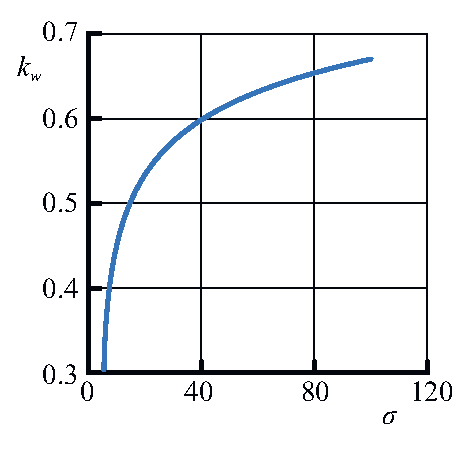
\includegraphics{101} %ширина рисунка составляет половину от ширины текста, picture1 - название файла с изображением, помещенного в папку Images
		\caption{В подписи к рисунку точка в конце не ставится}
	\end{figure}
	
\newpage

	\begin{center}
		\section{Экспериментальное исследование тепловой конвекции} 			% Название главы. Глава всегда начинается с новой страницы. Название добавляется в Содержание автоматически
	\end{center}

	\subsection{Введение} 	% Название подглавы

В этом пункте часть текста закомментирована.
	
\begin{comment} 			% Окружение комментария

Например в геологии рассматривается модель образования и движения литосферных плит, выхода пород на земную поверхность, а также извержения вулканов, которая предполагает наличие мантийных потоков внутри Земли.



Их развитие осуществляется под действием локальных градиентов температуры на границе мантии и ядра.
При описании этих процессов рассматривается модель конвекции от точечного источника тепла в средах с большим числом Прандтля.

\end{comment} 

\subsubsection{Формулы}		% Название подпункта

Формула в одну строку: $ a = b, b = c → \Rightarrow a = c $

«Выключная» формула, где\\ 
\textit{x} - обычный курсив;\\
$ x $ - математический курсив:

$$
 x^{333} + y^{333} = z^{333}
$$

\[
\int x^2 dx = \frac{x^3}{3} + g.
\]

Система уравнений:

\begin{equation}
\begin{cases}\renewcommand{\arraystretch}{2.}
\begin{array}{lcl}
x &=& \dfrac{1}{2}y, \\
y &=& \dfrac{x}{z}+1.
\end{array}
\end{cases}
\label{1}
\end{equation}

На пронумерованные формулы можно ссылаться в тексте (\ref{1}).

\newpage

	\begin{center} 	% Создание списка литературы в соотвествии со стилевым файлом ugost2008
		\bibliography{biblio} 	% biblio - название файла с библиографическим списком литературы
	\end{center}
	\addcontentsline{toc}{section}{Список литературы} % Добавляет Список литературы в Содержание

\end{document}
